\chapter{Cenni di Sicurezza di Rete}

\section{Introduzione}

Nel pieno dell'era digitale, si ha la necessità di memorizzare informazioni relative a ogni aspetto della nostra vita.\
L'informazione è divenuta una risorsa preziosa che deve essere protetta da qualsiasi possibile attacco.\
In particolare, è necessario proteggerla da accessi non autorizzati (\emph{riservatezza} o \emph{segretezza}) e da modifiche non autorizzate (\emph{integrità}), al fine di poterla rendere disponibile quando necessario alle entità autorizzate (\emph{accessibilità}).

Negli ultimi trent'anni le reti hanno creato una rivoluzione nell'uso dell'informazione, che risulta ora largamente distribuita:\ mediante le reti è possibile inviare e prelevare informazioni a distanza.\
In questo nuovo contesto i tre requisiti menzionati in precedenza - riservatezza, integrità e accessibilità - non sono cambiati, ma hanno acquisito nuove dimensioni.\
Non è più sufficiente garantire la riservatezza delle informazioni archiviate su qualche supporto ma deve essere possibile mantenerne la riservatezza anche quando vengono trasmesse da un computer all'altro.\
Pertanto è necessario garantire la sicurezza sia nel trasferimento dei dati sia della loro memorizzazione e conservazione.

\subsection{Obiettivi della sicurezza}

\subsubsection{\emph{Riservatezza}}

La \textit{riservatezza} (segretezza o confidenzialità) è probabilmente l'aspetto più evidente della sicurezza delle informazioni:\ è ovviamente necessario proteggere le informazioni considerate confidenziali.\
Un'organizzazione deve cautelarsi da possibili azioni ostili che mettano a rischio la riservetezza delle proprie informazioni, riservatezza che non è solamente relativa all'\textit{archiviazione} delle informazioni ma anche alla loro \textit{trasmissione}.\
Quando si trasmettono delle informazioni riservate con lo scopo di memorizzarle su un computer remoto o quando si prelevano le informazioni da un computer remoto, è necessario garantirne la protezione.

\subsubsection{\textit{Integrità}}

Le informazioni richiedono aggiornamenti continui.\
Se un cliente deposita o preleva denaro dal proprio conto in banca, il saldo deve essere immediatamente aggiornato.\
Garantire l'\textit{integrità} significa assicurare che le modifiche possano essere apportate esclusivamente dalle entità autorizzate e solo rispettando le procedure previste.

\subsubsection{\textit{Accessibilità}}

Il terzo aspetto relativo alla sicurezza delle informazioni è l'\textit{accessibilità}.\
L'informazione prodotta e archiviata da un'organizzazione deve essere resa disponibile alle entità autorizzate.\
Qualsiasi informazione diviene inutile se non è accessibile.\
Deve inoltre poter essere costantemente aggiornata, quindi sempre accessibile alle entità preposte.\
L'inaccessibilità dell'informazione è tanto dannosa per un'organizzazione quanto per la perdita di riservatezza o integrità delle informazioni.

\section{Sicurezza della comunicazione}

Una comunicazione in rete tra due entità può essere minata da vari tipi di attacchi, che possono essere raggruppati in base all'obiettivo dell'attacco.

\subsection{Attacchi}

\subsubsection{\textit{Attacchi alla riservatezza}}

In generale vi sono due tipi di attacchi che possono compromettere la riservatezza dell'informazione:\ l'\textit{intercettazione} e l'\textit{analisi del traffico}.

\paragraph{Intercettazione} L'\textit{intercettazione} si riferisce all'accesso non autorizzato ai dati o alla loro intercettazione durante la trasmissione.\
Per esempio un file trasferito tramite Internet potrebbe contenere informazioni confidenziali:\ un'entità non autorizzata potrebbe intercettarne la trasmissione e utilizzarne i contenuti per i propri scopi.\
Per contrastare l'intercettazione, i dati possono essere resi incomprensibili all'intercettatore utilizzando le tecniche di \textit{cifratura} che verranno discusse in seguito.

\subsubsection{\textit{Attacchi all'integrità}}

L'integrità dei dati può essere compromessa da vari tipi di attacchi:\ \textit{modifica}, \textit{masquerading}, \textit{ripetizione} e \textit{repudiation}.

\paragraph{Modifica} In questo caso l'attaccante modifica per i propri scopi le informazioni alle quali ha avuto accesso.\
Questo può avvenire per esempio quando un cliente invia un messaggio alla propria banca per disporre una transazione e l'attaccante intercetta il messaggio e modifica la transazione a proprio benificio.\
Si noti che in certi casi è sufficiente che l'attaccante elimini o semplicemente ritardi il messaggio per danneggiare il sistema o per trarne benifici personali.

\paragraph{Masquerading}

Si parla di \textit{masquerading} o \textit{spoofing} quando l'attaccante impersona (finge di essere) qualcun altro.\
Un noto attacco di masquerading è l'IP spoofing, in cui l'attaccante invia un messaggio a un computer indicando che il messaggio arriva da un'entità autorizzata.\
L'attaccante recupera prima l'indirizzo IP di un'entità autorizzata e poi modifica l'intestazione del pacchetto che invia inserendo l'indirizzo IP di quella entità invece che il proprio.\
In questo modo l'attaccante può impersonare un'entità autorizzata e ottenere diritti di accesso o redirezionare la vittima su un sito camuffato per carpire informazioni riservate.

\paragraph{Ripetizione} Nell'\textit{attacco a ripetizione} l'attaccante ottiene una copia del messaggio inviato da un utente per replicarlo in un momento successivo.\
Per esempio una persona invia alla propria banca una richiesta di pagamento a favore dell'attaccante che ha svolto un lavoro legittimo; questi intercetta il messaggio e ne invia una replica per ottenere un doppio pagamento dalla banca.

\paragraph{Repudiation} Questo tipo di attacco differisce dai precedenti perché viene sferrato da una delle parti in comunicazione, il mittente o il destinatario:\ il mittente di un messaggio potrebbe successivamente negare di averlo inviato o il destinatario di un messaggio potrebbe successivamente negare di averlo ricevuto.\
Un esempio di \textit{repudiation da parte del mittente} potrebbe essere il caso del cliente di una banca che ha chiesto di trasferire del denaro a una terza parte, ma nega in seguito di avere richiesto l'operazione.\
Un esempio di \textit{repudiation da parte del destinatario} potrebbe essere il caso in cui una persona acquista un prodotto da un'azienda pagandone regolarmente il corrispettivo, ma l'azienda nega successivamente di aver incassato il denaro chiedendo di ripetere il versamento.

\subsubsection{\textit{Attacchi all'accessibilità}}

Il più noto attacco all'accessibilità è il \textit{denial of service} (negazione del servizio).

\paragraph{Denial of service} Il \textit{denial of service} è una tipologia di attacco particolarmente diffusa, che può rallentare o interrompere il servizio di un sistema.\
Per raggiungere lo scopo l'attaccante ha a disposizione diverse strategie.\
Può inviare un numero di richieste fittizie talmente elevato da far crollare il sistema sotto il peso del traffico.\
Può intercettare ed eliminare le risposte del server a un client, facendo credere a quest'ultimo che il server non sia operativo.\
Può anche intercettare le richieste dei client, inducendoli a inviare più richieste e sovraccarricare il sistema.

\subsection{Cifratura a chiave simmetrica}

La cifratura a chiave simmetrica garantisce la riservatezza dei dati.\
Nella cifratura a chiave simmetrica si utilizza la medesima chiave sia per l'operazione di cifratura che per quella di decifratura; la chiave può essere utilizzata per la comunicazione bidirezionale.\
Per tali motivi questo tipo di cifratura, illustrata nella Figura \ref{fig:cifratura_simmetrica}, viene chiamata \textit{simmetrica}.

\begin{center}
    Le tecniche di cifratura a chiave simmetrica sono anche chiamate a chiave segreta.
\end{center}
\begin{figure}[H]
    \centering
    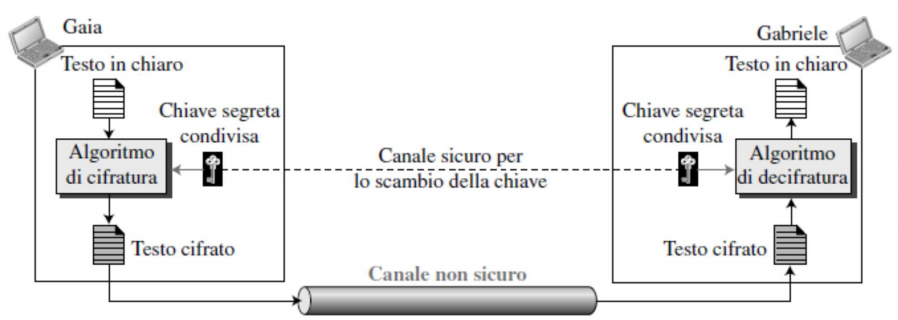
\includegraphics[width=0.7\textwidth]{immagini/Cifratura_simmetrica.png}
    \caption{L'idea generale della cifratura a chiave simmetrica}
    \label{fig:cifratura_simmetrica}
\end{figure}
Nella Figura \ref{fig:cifratura_simmetrica} un'entità, Gaia, invia un messaggio a un'altra entità, Gabriele, su un canale insicuro; grazie alla crittografia un avversario, Eva, non può comprendere i contenuti del messaggio ascoltando semplicemente il canale.

Il messaggio originale da Gaia a Gabriele è chiamato \textit{testo in chiaro} (\textit{plaintext}), il messaggio inviato attraverso il canale è chiamato \textit{testo cifrato} (\textit{ciphertext}).\
Per ottenere il testo cifrato dal testo in chiaro, Gaia utilizza un \textit{algoritmo di cifratura} (o algoritmo crittografico) e una \textit{chiave segreta} condivisa.\
Per ottenere il testo in chiaro dal testo cifrato Gabriele utilizza un \textit{algortimo di decifratura} e la medesima chiave segreta.\
La chiave è costituita da un insieme di valori (numeri) utilizzati dai due algoritmi.

\subsubsection{Algoritmi crittografici a sostituzione}

Un cifrario a sostituzione sostituisce un simbolo del testo in chiaro con un altro simbolo.\
Se i simboli del testo in chiaro sono caratteri, si rimpiazza un carattere con un altro.\
Gli algoritmi crittografici a sostituzione possono essere classificati in \textit{monoalfabetici} o \textit{polialfabetici}.
\begin{itemize}
    \item \textbf{Cifrari monoalfabetici}:\ ogni carattere (o simbolo) nel testo in chiaro viene sempre sostituito dallo stesso carattere (o simbolo) nel testo cifrato indipendentemente dalla posizione nel testo.
    \item \textbf{Cifrari polialfabetici}:\ le diverse occorrenze dello stesso carattere possono corrispondere a un sostituto differente:\ la relazione fra un carattere nel testo in chiaro e il carattere corrispondente nel testo cifrato è di uno-a-molti.\
          I cifrari polialfabetici hanno il vantaggio di nascondere la frequenza delle singole lettere per violare il testo cifrato.
\end{itemize}

\subsubsection{\textit{Cifrari moderni a chiave simmetrica}}

I cifrari a chiave simmetrica tradizionali operano a livello di caratteri, ma l'avvento dei computer rende preferibile l'impiego di cifrari orientati al bit.

\paragraph{\textit{Cifrari moderni a blocchi}} Un cifrario simmetrico moderno a blocchi cifra un blocco di \textit{n} bit di testo in chiaro o decifra un blocco di \textit{n} bit di testo cifrato.\
In un cifrario di questo tipo un blocco di testo cifrato dipende dall'intero blocco di testo in chiaro.\
Gli algoritimi di cifratura e decifratura usano una chiave di \textit{k} bit e devono essere l'uno l'inverso dell'altro.

\begin{itemize}
    \item \textbf{\textit{DES:\ Data Encryption Standard}} $\rightarrow$ chiave di cifratura 56 bit
    \item \textbf{\textit{AES:\ Advanced Encryption Standard}}
          \begin{itemize}
              \item 2001 standard, sostituisce DES
              \item Elabora dati in blocchi di 128 bit, chiave di 128, 192, o 256 bit
          \end{itemize}
\end{itemize}

\subsubsection{Problemi}

\begin{itemize}
    \item Come si accordano A e B su chiave da usare? (soprattutto se non si incontrano mai?)
    \item Segretezza chiave inversamente proporzionale a quanto viene usata.
\end{itemize}

\subsection{Cifratura a chiave asimmetrica}

Nel caso della crittografia simmetrica l'informazione segreta (la chiave) deve essere condivisa fra due persone.\
Nel caso della crittografia asimmetrica l'informazione segreta è personale (non condivisa):\ ciascuna persona crea e conserva privatamente la propria informazione riservata.

Mentre la cifratura simmetrica si basa sulla sostituzione e sulla permutazione di simboli (caratteri o bit), la crittografia asimmetrica si basa sull'applicazione di funzioni matematiche a numeri.\
Nella crittografia simmetrica il testo in chiaro e il testo cifrato sono considerati una combinazione di simboli, la cifratura e la decifratura permutano questi simboli o li costituiscono con altri.\
Nella crittografia asimmetrica, invece, il testo in chiaro e il testo cifrato sono considerati numeri; la cifratura e la decifratura sono funzioni matematiche applicate a numeri che consentono di otterne altri.

La crittografia a chiave asimmetrica impiega due chiavi separate:\ una privata e una pubblica.

\subsubsection{\textit{L'idea generale}}

\begin{figure}[H]
    \centering
    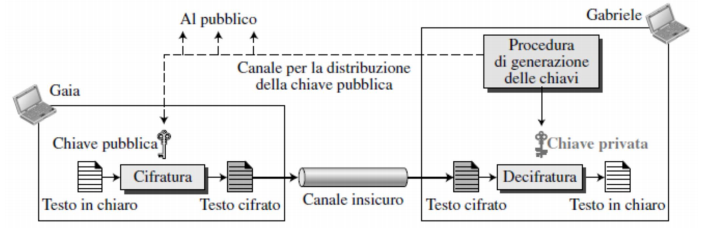
\includegraphics[width=0.7\textwidth]{immagini/Cifratura_asimmetrica.png}
    \caption{L'idea generale della crittografia asimmetrica}
    \label{fig:cifratura_asimmetrica}
\end{figure}
La Figura \ref{fig:cifratura_asimmetrica} schematizza l'idea generale della crittografia assimetrica nel caso della cifratura.\
La figura evidenzia alcuni fatti importanti.\
In primo luogo pone in risalto la natura asimmetrica del cifrario.\
La responsabilità di garantire la sicurezza ricade principalmente sul destinatario (Gabriele in questo caso) che deve creare due chiavi:\ una privata e una pubblica.\
Gabriele ha il compito di distribuire la propria chiave pubblica alla comunità, per esempio tramite un canale di distribuzione della chiave pubblica.\
Sebbene questo canale non debba assicurare la riservatezza, deve garantire autenticazione e integrità.\
Eva non deve poter pubblicizzare la propria chiave pubblica alla comunità sostenendo che si tratti della chiave pubblica di Gabriele.

In secondo luogo la crittografia asimmetrica implica che Gabriele e Gaia non possano utilizzare la stessa coppia di chiavi per la comunicazione bidirezionale; ciascun membro della comunità deve creare la propria coppia di chiavi pubblica e privata.\
La Figura \ref{fig:cifratura_asimmetrica} illustra come Gaia possa utilizzare la chiave pubblica di Gabriele per inviare messaggi crittografati a Gabriele; se Gabriele volesse rispondere, Gaia dovrebbe stabilire la propria coppia di chiavi pubblica e privata.

Infine, la crittografia asimmetrica comporta che Gabriele abbia bisogno di una sola chiave privata per poter ricevere comunicazioni da qualsiasi membro della comunità, mentre Gaia deve utilizzare \textit{n} chiavi pubbliche per poter comunicare con \textit{n} membri della comunità, una per ciascuna di essi.\
In altre parole Gaia deve utilizzare un \textit{key ring} (mazzo di chiavi).

Lo svantaggio della cifratura asimmetrica è l’efficienza, per questa ragione viene usata generalmente per messaggi di dimensione ridotta.\
È importante sapere che per usufruire di tutte le funzionalità di sicurezza più avanzate, sono necessarie entrambe le tecniche di crittografia, che sono complementari fra loro.

Esempio di cifratura asimmetrica:\ RSA.

\subsection{Message digest}

Vi sono casi in cui pur non essendo richiesta la riservatezza, risulta di fondamentale importanza l'\textit{integrità}:\ il messaggio originale non deve poter essere modificato.\
Gaia potrebbe per esempio scrivere un documento che non necessita di segretezza (dunque non deve essere cifrato), ma che deve rimanere integro, ovvero il suo contenuto non può essere modificato.

Un modo per preservare l'integrità è quella di inviare insieme al messaggio un codice generato dal mittente e dipendente dal messaggio.\
Questo codice viene elaborato con un particolare algoritmo chiamato \textit{funzione hash crittografica}.\
Questa funzione crea un'immagine compressa del messaggio.\
Gabriele, per verificare che il messaggio ricevuto non sia stato modificato, applica la funzione hash crittografica al messaggio ricevuto e confronta il nuovo digest con quello inviato da Gaia:\ se risultano identici Gabriele ha la garanzia che il messaggio originale non è stato modificato.\
La Figura \ref{fig:digest} illustra questa tecnica.\
Ovviamente non deve essere possibile modificare il digest del messaggio.

\begin{figure}[H]
    \centering
    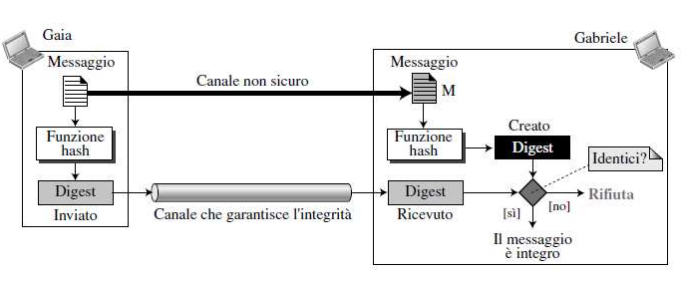
\includegraphics[width=0.8\textwidth]{immagini/Message_digest.png}
    \caption{Messaggio e relativo digest}
    \label{fig:digest}
\end{figure}

Si noti che il digest dipende dal messaggio ma viene inviato separatamente, per cui il messaggio viaggia in chiaro e non è preservata la confidenzialità, che invece richiede l'applicazione di meccanismi di crittografia.

\textbf{Funzione hash}:\ riceve un messaggio di lunghezza arbitraria e produce un digest di lunghezza fissa.\
Esempi:\ MD4, MD5, SHA\dots

\subsection{Message Authentication Code}

Il digest può essere utilizzato per verificare l'integrità di un messaggio - ovvero per verificare che il messaggio non sia stato modificato.\
Per garantire anche l'\textit{autenticazione} del messaggio - ovvero garantire che Gaia, non qualcun altro, abbia originato il messaggio - è necessario includere nel processo un'informazione segreta condivisa da Gaia e Gabriele (che Eva non possiede):\ si deve creare un codice MAC (\textit{Message Authentication Code}).\
La Figura \ref{fig:MAC} illustra l'idea.

\begin{figure}[H]
    \centering
    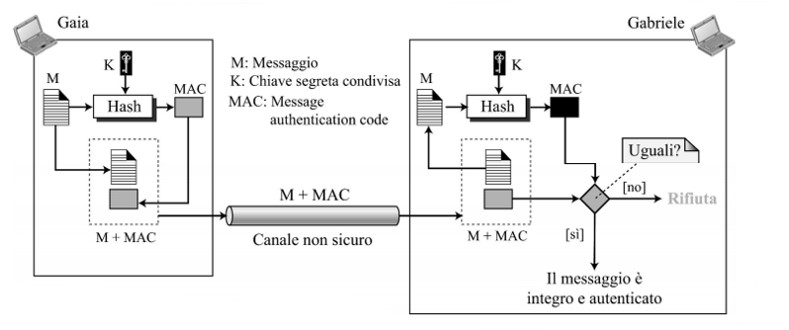
\includegraphics[width=0.7\textwidth]{immagini/MAC.jpg}
    \caption{Codice di autenticazione di messaggio (MAC)}
    \label{fig:MAC}
\end{figure}

Gaia e Gabriele condividono la chiave segreta K.\
Gaia crea un MAC applicando la funzione hash alla concatenazione della chiave segreta e del messaggio \textit{h}(K + M).\
Gaia invia il messaggio e il relativo MAC a Gabriele tramite il canale insicuro.\
Gabriele separa il messaggio dal MAC ed elabora un nuovo MAC dalla concatenazione della chiave segreta e del messaggio ricevuto.\
Confronta infine il MAC così ottenuto con il MAC ricevuto:\ se sono identici il messaggio è autentico e non è stato modificato.

Si noti che in questo caso non è necessario usare due canali:\ sia il messaggio sia il MAC possono essere inviati sullo stesso canale insicuro.\
Eva può vedere il messaggio ma non può formularne uno nuovo per sostituire il precedente poiché non possiede la chiave segreta condivisa da Gaia e Gabriele.\
Eva non può creare lo stesso MAC ottenuto da Gaia.

\subsection{Firma digitale}

Un altro modo per garantire l'integrità e l'autenticazione di un messaggio è la \textit{firma digitale}.\
Il MAC utilizza una chiave segreta per proteggere il digest, mentre la firma digitale utilizza una coppia di chiavi pubblica-privata.

Quando Gaia invia un messaggio a Gabriele, questi può voler verificare l'autenticità del mittente, ovvero può richiedere garanzie che il messaggio provenga da Gaia e non da Eva:\ in questo caso può quindi chiedere a Gaia di firmare elettronicamente il messaggio.\
In altri termini la firma elettronica può provare l'autenticità di Gaia come mittente del messaggio.\
Questo tipo di firma viene chiamata \textit{firma digitale}.

\subsubsection{\textit{Funzionamento}}

Gaia firma il messaggio M cifrandolo con la sua chiave privata.\
La cifratura del messaggio M costituisce proprio la firma S di Gaia (solo Gaia conosce la sua chiave privata).\
A questo punto Gaia invia sia il messaggio M sia la firma S a Gabriele, il quale verifica l'autenticità del messaggio applicando la chiave pubblica di Gaia.\
Se il messaggio che Gabriele ottiene è uguale a quello inviato da Gaia allora il messaggio è autentico.

Si noti che quando il documento è firmato, chiunque, Gabriele incluso, può verificarne la firma poiché la chiave pubblica di Gaia è di dominio pubblico.\
Gaia non deve invece utilizzare la propria chiave pubblica per firmare il documento altrimenti la propria firma potrebbe essere forgiata da chiunque.

È possibile utilizzare una chiave segreta (simmetrica) sia per firmare che per verificare una firma? La risposta è negativa per varie ragioni.\
Per prima cosa una chiave segreta è nota solo a due entità (Gabriele e Gaia nell'esempio).\
Quindi se Gaia dovesse firmare un altro documento da inviare a Filippo, dovrebbe utilizzare un'altra chiave segreta.\
Secondo creare una chiave segreta per una sessione comporta l'autenticazione, che a sua volta utilizza la firma digitale:\ si cadrebbe così in un circolo vizioso.\
Terzo, Gabriele potrebbe utilizzare la chiave segreta condivisa con Gaia per firmare un documento da inviare a Filippo e sostenere che il documento proviene da Gaia.

Si dovrebbe fare una distinzione fra l'impiego delle chiavi pubblica e privata nella firma digitale rispetto al loro impiego nei sistemi crittografici per garantire la riservatezza.\
In quest'ultimo caso vengono utilizzate le chiavi pubbliche e private del destinatario:\ il mittente utilizza una chiave pubblica del destinatario per crittografare, quest'ultimo utilizza la propria chiave privata per decifrare.\
Nella firma digitale vengono invece impiegate le chiavi pubblica e privata del mittente:\ quest'ultimo utilizza la propria chiave privata per firmare il messaggio, il destinatario utilizza la chiave pubblica del mittente per verificare l'autenticità del messaggio.

\paragraph{Non-repudiation} Se Gaia firmasse un messaggio ma successivamente negasse di averlo fatto, Gabriele potrebbe provare il contrario? Con lo schema considerato fino a questo momento Gabriele potrebbe trovarsi in difficoltà nel garantire l'autenticità a distanza di tempo.\
Dovrebbe conservare la firma in archivio e successivamente utilizzare la chiave pubblica di Gaia per creare il messaggio originale provando che il messaggio in archivio e il messaggio così creato sono identici.\
Questo non è in realtà fattibile poiché Gaia potrebbe nel frattempo aver sostituito le proprie chiavi, e potrebbe sostenere che l'archivio contenente la firma non è autentico.

Una possibile soluzione consiste nel fare intervenire una terza parte fidata, che faccia da tramite da Gaia e Gabriele al fine di garantire che i messaggi inviati non possano essere disconosciuti dal mittente.

\section{Comunicazione sicure nello stack protocollare}

\subsection{Sicurezza al livello rete:\ IPSec}

È necessario garantire la sicurezza anche al livello di rete perché ci sono programmi applicativi che non implementano meccanismi di sicurezza o che sfruttano servizi di UDP.\
Inoltre numerose applicazioni, tra cui i protocolli di routing, usano direttamente i servizi di IP.\
Tutte queste applicazioni richiedono dunque servizi di sicurezza a livello rete.

IPSec (o IPSecurity) è un insieme di protocolli sviluppato dall'IETF (Internet Engineering Task Force) per fornire garanzie di sicurezza ai pacchetti di livello rete.\
IPSec serve ad autenticare e rendere confidenziali i pacchetti del protocollo IP.\
IPSec può operare in due modi:\ in \textit{modalità trasporto} o in \textit{modalità tunnel}.
\begin{figure}[H]
    \centering
    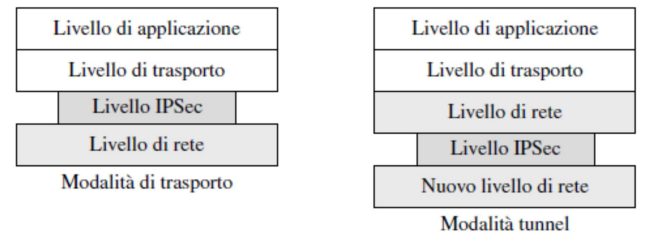
\includegraphics[width=0.7\textwidth]{immagini/IPSec.png}
\end{figure}

\paragraph{\textit{Modalità traporto}}

Nella modalità traporto, IPSec protegge ciò che viene fornito dal livello trasporto al livello rete.\
In altre parole, questa modalità protegge i dati incapsulati nei pacchetti di livello rete, come rappresentato nella Figura \ref{fig:traporto}.

\begin{figure}[H]
    \centering
    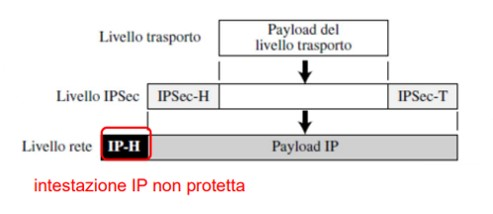
\includegraphics[width=0.6\textwidth]{immagini/mod_trasporto.jpg}
    \caption{IPSec in modalità trasporto.}
    \label{fig:traporto}
\end{figure}
Si noti che la protezione è solo sui dati, ovvero sul payload dal livello trasporto:\ l'intestazione del pacchetto IP non viene protetta.\
L'intestazione (e il trailer) di IPSec vengono aggiunti ai dati provenienti dal livello trasporto prima dell'intestazione IP.

La modalità trasporto viene normalmente utilizzata quando occorre proteggere i dati scambiati fra mittente e destinatario (end-to-end).\
L'host mittente sfrutta il protocollo IPSec per autenticare e/o cifrare i dati consegnati dal livello traporto.\
L'host destinatario sfrutta il protocollo IPSec per verificare l'autenticità dei dati e/o decifrarli, per poi consegnarli al livello trasporto.

\paragraph{\textit{Modalità tunnel}}

Nella modalità tunnel IPSec permette di proteggere l'intero pacchetto IP.\
Con questa modalità l'intero pacchetto IP, inclusa l'intestazione, viene incapsulato in un pacchetto IPSec.\
Il tutto deve essere poi inserito in un pacchetto IP:\ verrà quindi aggiunta una nuova intestazione IP, come mostrato nella Figura \ref{fig:tunnel}.

\begin{figure}[H]
    \centering
    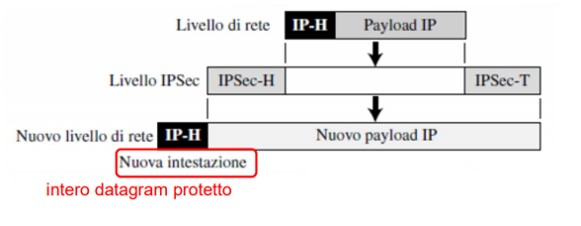
\includegraphics[width=0.7\textwidth]{immagini/mod_tunnel.jpg}
    \caption{IPSec in modalità tunnel.}
    \label{fig:tunnel}
\end{figure}
La nuova intestazione è diversa dall'intestazione IP iniziale.\
La modalità tunnel viene solitamente utilizzata fra due router, fra un host e un router o fra un router un host.\
L'intero pacchetto originale viene protetto da intrusioni fra il mittente e il destinatario, come se il pacchetto viaggiasse in un tunnel immaginario.

\subsubsection{\textit{Protocollo ESP}}

ESP (Encapsulating Security Protocol) è un protocollo di IPSec che fornisce autenticazione di sorgente, integrità e riservatezza.\
Il protocollo ESP aggiunge un'intestazione e un trailer, come mostrato nella Figura \ref{fig:ESP}.

\begin{figure}[H]
    \centering
    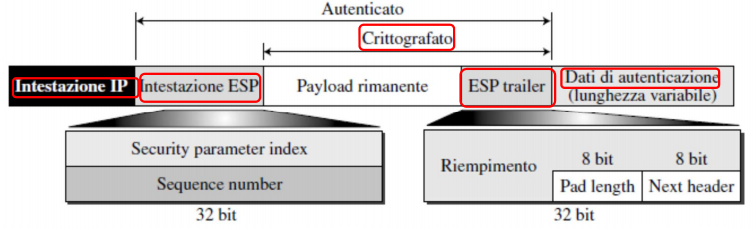
\includegraphics[width=0.7\textwidth]{immagini/ESP.png}
    \caption{Protocollo ESP}
    \label{fig:ESP}
\end{figure}

Si noti che i dati di autenticazione ESP sono aggiunti in coda al pacchetto, per facilitarne il calcolo.\
Quando un datagramma IP trasporta un pacchetto ESP, il valore del campo protocollo dell'intestazione IP è 50.\
Il campo next header nel trailer di ESP specifica il protocollo originale (il tipo di pacchetto contenuto dal datagramma IP, per esempio TCP o UDP).\
Ecco come avviene la formazione del pacchetto ESP:

\begin{enumerate}
    \item il trailer ESP viene aggiunto al payload;
    \item payload e trailer vengono crittografati;
    \item viene aggiunta l'intestazione ESP;
    \item intestazione ESP, payload ed ESP trailer vengono usati per generare i dati di autenticazione;
    \item i dati di autenticazione vengono aggiunti al termine del trailer ESP;
    \item viene aggiunta un'intestazione IP dopo averne impostato il valore del campo protocollo a 50.
\end{enumerate}

\subsubsection{\textit{Reti private virtuali (VPN)}}

Una delle applicazioni di IPSec è nelle \textit{reti private virtuali}.\
Una rete privata virtuale (Virtual Private Network, o VPN) è una tecnologia sempre più utilizzata dalle aziende che adottano Internet per le comunicazioni interne ed esterne, ma che richiedono riservatezza nelle comunicazioni.\
Una VPN è una rete che è privata ma virtuale:\ privata perché garantisce la riservatezza all'organizzazione, virtuale poiché non utilizza realmente dei collegamenti WAN privati.\
La rete è fisicamente pubblica ma virtualmente privata.\
La Figura \ref{fig:VPN} illustra il concetto di rete privata virtuale.

\begin{figure}[H]
    \centering
    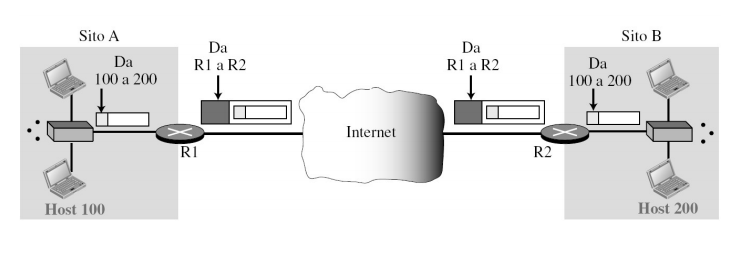
\includegraphics[width=0.8\textwidth]{immagini/VPN.png}
    \caption{Una rete privata virtuale (VPN)}
    \label{fig:VPN}
\end{figure}
I router R1 e R2 usano la tecnologia VPN per garantire la riservatezza all'organizzazione.\
La tecnologia VPN impiega il protocollo ESP di IPSec in modalità tunnel:\ il datagramma privato, inclusa la sua intestazione, viene incapsulato in un pacchetto ESP.\
Il router al confine del sito mittente usa nel nuovo datagramma il proprio indirizzo IP e l'indirizzo IP del router nel sito destinatario.\
La rete pubblica (Internet) è responsabile del trasporto del pacchetto da R1 e R2.\
Eventuali osservatori esterni non possono decifrare i contenuti del pacchetto e nemmeno gli indirizzi mittente e destinatario.\
La decifratura avviene in R2, che identifica l'indirizzo di destinazione del pacchetto e lo inoltra.
